\documentclass[journal]{IEEEtran}
\usepackage{amsmath,amssymb}
\usepackage{graphicx}
\usepackage{booktabs}
\usepackage{multirow}
\usepackage{xcolor}
\usepackage[hidelinks]{hyperref}
\graphicspath{{figures/}}

% Every number in the results is generated from ml_pipeline/runs/*.json by paper/make_tables.py
% (tables/*.tex and the macros in tables/numbers.tex). Re-run that script; never edit numbers by hand.
\newcommand{\hzPT}{22.06}
\newcommand{\hzPTstd}{0.09}
\newcommand{\hzP}{21.72}
\newcommand{\hzPV}{23.85}
\newcommand{\hzPVstd}{0.10}
\newcommand{\hzPVpaper}{23.79}
\newcommand{\hzRidge}{25.96}
\newcommand{\shPT}{24.09}
\newcommand{\shPTstd}{0.03}
\newcommand{\shPV}{27.44}
\newcommand{\shPVstd}{0.23}
\newcommand{\shPVpaper}{24.77}
\newcommand{\shRidge}{25.62}
\newcommand{\hzPVvalHund}{24.40}
\newcommand{\hzPVval}{22.53}
\newcommand{\hzGain}{7.5}
\newcommand{\shGain}{12.2}
\newcommand{\shGainPaper}{2.7}
\newcommand{\hzGainFifteen}{4.4}
\newcommand{\hzGainSixty}{9.6}
\newcommand{\shHolPT}{24.49}
\newcommand{\shHolPV}{21.48}
\newcommand{\shMakePT}{33.69}
\newcommand{\shMakePV}{29.41}
\newcommand{\shWorkPT}{24.48}
\newcommand{\shWorkPV}{29.61}


\begin{document}

\title{Remembering Yesterday: Periodicity- and Calendar-Aware Physical-Virtual Graph Networks for Metro Ridership Forecasting}

\author{Nitin~Bharti% TODO: add supervisor / co-authors and affiliation
\thanks{Code, data pipeline and all run logs: TODO(repository URL).}}

\maketitle

\begin{abstract}
Station-level metro ridership forecasting models such as the Physical-Virtual Collaboration Graph Network (PVCGN) predict the next hour from the last hour of ridership only, without any notion of time of day, day type or earlier days. On the public HZMetro and SHMetro benchmarks we show that this discards the strongest available signal: ridership at the same time on the most recent comparable day correlates at $r\approx0.96$--$0.99$ with ridership one hour ahead, versus $r\approx0.66$--$0.70$ for the most recent observation. We propose PT-PVCGN, which adds periodic reference inputs (the same time slots on the most recent day of the same working/non-working type and on the same weekday a week earlier) and calendar embeddings to PVCGN, and which reduces exactly to PVCGN when both are disabled. With a numerically verified re-implementation of PVCGN, identical splits and metrics, equal training budgets, multiple seeds and a single held-out test evaluation, PT-PVCGN lowers test MAE on HZMetro from \hzPV{} to \hzPT{} (\hzGain\% lower), with the gain growing from \hzGainFifteen\% at 15 minutes to \hzGainSixty\% at 60 minutes. On SHMetro, after only 30 training epochs, it reaches a test MAE of \shPT{}, below both our equally trained PVCGN (\shPV{}) and the PVCGN result reported after 200 epochs (\shPVpaper). The ablation shows that the periodic inputs carry the improvement while the calendar embeddings add nothing, and error analysis reveals a clear weakness on public holidays and make-up working days.
\end{abstract}

\begin{IEEEkeywords}
Metro ridership prediction, graph neural networks, periodicity, calendar effects, spatio-temporal forecasting.
\end{IEEEkeywords}

\section{Introduction}
\IEEEPARstart{A}{ccurate} short-term forecasts of station inflow and outflow support train dispatching, crowd control and passenger information in large metro systems. Graph neural networks have become the dominant approach because they respect the irregular topology of a metro network~\cite{li2018dcrnn,wu2019graphwavenet}. Among them, PVCGN~\cite{liu2022pvcgn} constructs three complementary graphs---a physical graph from the line topology, a similarity graph from dynamic-time-warping distances between station flow series, and a correlation graph from historical origin-destination (OD) ratios---and embeds them in a graph-convolutional gated recurrent unit within a sequence-to-sequence model.

PVCGN, like many station-level models, forecasts the next hour from only the previous hour of observations and has no notion of time of day, day of week or public holidays. Its authors explicitly name the periodic evolution of ridership as future work~\cite{liu2022pvcgn}. An exploratory analysis of the released benchmarks shows that this is the dominant long-horizon signal: ridership at the same slot on a comparable earlier day explains far more of the 60-minute-ahead ridership than the latest observation (Fig.~\ref{fig:lags}), and weekday and weekend daily profiles differ sharply (Fig.~\ref{fig:profile}).

We make the following contributions:
\begin{enumerate}
\item A data analysis of HZMetro and SHMetro that quantifies the periodic structure ignored by PVCGN, including calendar effects (a public holiday and an official make-up working Sunday in the SHMetro test period).
\item PT-PVCGN, a minimal extension of PVCGN with periodic reference-day inputs (P) and calendar embeddings (T), which reduces exactly to PVCGN when both are disabled.
\item A controlled evaluation: a re-implementation of PVCGN verified against the authors' code and reproducing their HZMetro test MAE (\hzPV{} vs.\ \hzPVpaper{} reported), equal training budgets, seasonal and lag-feature baselines that were missing from the original comparison, multiple seeds, and a single test evaluation of a pre-registered set of models.
\item An ablation and error analysis showing that the periodic inputs carry the gain, that calendar embeddings do not help, and that periodic references mislead the model on irregular calendar days.
\end{enumerate}

\section{Related Work}
\textbf{Graph-based traffic forecasting.} DCRNN~\cite{li2018dcrnn} models traffic as diffusion on a road graph inside a sequence-to-sequence GRU; Graph WaveNet~\cite{wu2019graphwavenet} learns an adaptive adjacency matrix; ASTGCN~\cite{guo2019astgcn} adds spatial-temporal attention and explicitly models recent, daily and weekly components; ST-MGCN~\cite{geng2019stmgcn} fuses several hand-designed graphs for ride-hailing demand.
\textbf{Metro ridership.} PVCGN~\cite{liu2022pvcgn} introduced the SHMetro and HZMetro benchmarks and physical-virtual graph collaboration. TODO: add 2022--2026 metro ridership works after a literature search, and verify every citation against the original paper.
\textbf{Periodicity.} Periodic components are standard in grid-based crowd-flow models~\cite{zhang2017stresnet,yao2019stdn} and in ASTGCN~\cite{guo2019astgcn}, and temporal embeddings are used in attention-based models such as GMAN~\cite{zheng2020gman}. Our contribution is to add calendar-aware periodicity, in a controlled and ablatable way, to a strong metro-specific multi-graph model and to measure its value against the original model and against strong periodic non-neural baselines under identical protocols.

\section{Problem Definition}
Let $\mathbf{X}_t\in\mathbb{R}^{N\times 2}$ be the inflow and outflow of $N$ stations in 15-minute interval $t$. Given observations up to $t$ and the public calendar, the task is to predict $\hat{\mathbf{X}}_{t+1},\dots,\hat{\mathbf{X}}_{t+4}$ (15 to 60 minutes ahead). Following~\cite{liu2022pvcgn}, forecasts are issued every 15 minutes during service hours (66 origins per day). Each day $d$ is labelled working or non-working using the official calendar, including public holidays and make-up working days.

\section{Method}
\subsection{PVCGN recap}
PVCGN encodes the last $n=4$ intervals with two stacked Collaborative Gated Recurrent Modules (CGRMs) and decodes four steps autoregressively. Each CGRM combines a graph-convolutional GRU, whose gates use a relational graph convolution
\begin{equation}
f(\mathbf{h}_i)=\Theta_0\mathbf{h}_i+\sum_{r\in\{p,s,c\}}\sum_{j}M_r(i,j)\,\Theta_r\mathbf{h}_j,
\label{eq:rgcn}
\end{equation}
with row-normalised physical, similarity and correlation matrices $M_r$ and basis-decomposed weights $\Theta_r$, and a fully connected GRU over all stations that provides global context.

\subsection{Periodic reference inputs (P)}
For a forecast on day $d$ we define two reference days that are strictly earlier than $d$: $d^{\text{type}}$, the most recent day with the same working/non-working label, and $d^{\text{week}}$, the same weekday one week earlier if it has the same label (otherwise $d^{\text{type}}$). At encoder step $k$ (slot $s$) the input of station $i$ is extended with $\mathbf{X}^{i}_{d^{\text{type}},s}$ and $\mathbf{X}^{i}_{d^{\text{week}},s}$; at decoder step $h$ the same is done for the target slot. The decoder therefore sees ``what usually happens next'' while the encoder sees how today deviates from the reference so far. Only past observations are used.

\subsection{Calendar embeddings (T)}
Learned embeddings of the time-of-day slot (16-d), day of week (4-d) and working-day flag (4-d) are concatenated to every node input at every step.

With P and T disabled the model is exactly PVCGN; P and T add 3.5\% parameters (38.9\,M vs.\ 37.6\,M on HZMetro) and no measurable training cost per epoch.

\section{Experimental Setup}
\textbf{Data.} HZMetro (80 stations, Jan 2019) and SHMetro (288 stations, Jul--Sep 2016) with the released chronological splits and graphs~\cite{liu2022pvcgn}. The HZMetro validation days are a weekend, while its test days are weekdays; the SHMetro test period contains the Mid-Autumn holiday (Sep 15--17) and a make-up working Sunday (Sep 18). Training days without an earlier reference day (the first two of each dataset) are excluded for all models.
\textbf{Re-implementation.} We re-implemented PVCGN in PyTorch without external graph libraries and verified that, given identical weights, its forward pass matches the authors' code to $10^{-5}$.
\textbf{Training.} All deep models follow the released PVCGN configuration (256 hidden units, two layers, Adam, learning rate $10^{-3}$, gradient clipping 5, L1 loss, curriculum learning) and differ only in P and T. On HZMetro every deep model uses the paper's 200-epoch schedule (learning rate $\times0.1$ at epochs 100 and 150, early stopping after 50 epochs without improvement) with 3 seeds. A shorter 100-epoch schedule is reported as a sensitivity check (Table~\ref{tab:ablation}): it under-trains PVCGN (validation MAE \hzPVvalHund{} vs.\ \hzPVval{} with 200 epochs). On SHMetro, compute limits (a single Apple M1 laptop; about 11 minutes per epoch) restrict both PVCGN and PT-PVCGN to 30 epochs (decay at 20 and 25) with 2 seeds. The epoch of each run is selected on validation MAE.
\textbf{Baselines.} Persistence; seasonal naive forecasts from the same-type reference day and from the weekly reference; historical average per station, slot and day type; ridge regression and histogram gradient boosting (one model per horizon and direction) on the last four observations, the reference-day values and calendar features; and PVCGN. For context we also quote the test results reported in~\cite{liu2022pvcgn}.
\textbf{Metrics.} MAE, RMSE and MAPE over non-zero targets, computed exactly as in the code of~\cite{liu2022pvcgn}, per horizon; additionally on rush hours (07:30--09:30, 17:30--19:30), the busiest quarter of stations by training ridership, and calendar slices.
\textbf{Protocol.} All decisions---the training budgets, the epoch of each run, and the choice of PT-PVCGN as the proposed model---were made on validation data. The test set of each city was then evaluated once, for all pre-registered models together.

\section{Results}
\subsection{Main results}
Tables~\ref{tab:hz} and~\ref{tab:sh} and Fig.~\ref{fig:test} report the test results. Our re-trained PVCGN reproduces the published HZMetro result (MAE \hzPV$\pm$\hzPVstd{} vs.\ \hzPVpaper{} reported), which validates the comparison. Under the same 200-epoch schedule, PT-PVCGN reduces the HZMetro test MAE to \hzPT$\pm$\hzPTstd{} (\hzGain\% lower), and it is more accurate at every horizon, RMSE and MAPE included. As expected from the analysis in the introduction, the benefit grows with the forecast horizon: \hzGainFifteen\% at 15 minutes and \hzGainSixty\% at 60 minutes, where the last observation is least informative and the periodic reference most informative.

On SHMetro, PT-PVCGN reaches \shPT$\pm$\shPTstd{} after 30 epochs, \shGain\% below our PVCGN trained for the same 30 epochs (\shPV$\pm$\shPVstd) and \shGainPaper\% below the PVCGN result reported after 200 epochs (\shPVpaper). Because our SHMetro budget is much shorter than the original one, we regard the SHMetro numbers as evidence that the gain carries over to a larger network rather than as a fully converged comparison.

The non-neural baselines are informative. A ridge regression on the last hour plus reference-day values (MAE \hzRidge{} on HZMetro, \shRidge{} on SHMetro) beats all seasonal baselines and, on SHMetro, our 30-epoch PVCGN; on HZMetro rush hours it is also better than PVCGN (Table~\ref{tab:slices}). Periodic information is therefore worth at least as much as the graph architecture, and adding it to the architecture gives the best of both.

\begin{table*}[t]
\centering
\caption{Test results on HZMetro (mean $\pm$ std over 3 seeds for trained deep models; all deep models use the same 200-epoch schedule). Baselines are deterministic.}
\label{tab:hz}
\scriptsize
\setlength{\tabcolsep}{3pt}
\begin{tabular}{lcccccccccccc}
\toprule
 & \multicolumn{3}{c}{15 min} & \multicolumn{3}{c}{30 min} & \multicolumn{3}{c}{45 min} & \multicolumn{3}{c}{60 min} \\
\cmidrule(lr){2-4} \cmidrule(lr){5-7} \cmidrule(lr){8-10} \cmidrule(lr){11-13}
Method & MAE & RMSE & MAPE & MAE & RMSE & MAPE & MAE & RMSE & MAPE & MAE & RMSE & MAPE \\
\midrule
Persistence & 43.78 & 81.78 & 22.23\% & 64.75 & 124.96 & 33.16\% & 86.47 & 167.01 & 50.84\% & 105.07 & 200.73 & 84.63\% \\
Historical average & 30.01 & 53.89 & 15.81\% & 30.03 & 53.86 & 15.93\% & 29.96 & 53.75 & 16.12\% & 29.83 & 53.65 & 16.55\% \\
Seasonal naive (same-type day) & 27.98 & 52.17 & 16.43\% & 28.03 & 52.21 & 16.71\% & 27.98 & 52.17 & 17.09\% & 27.90 & 52.16 & 17.70\% \\
Seasonal naive (weekly) & 31.14 & 51.42 & 17.91\% & 31.15 & 51.40 & 18.06\% & 31.07 & 51.31 & 18.27\% & 30.94 & 51.22 & 18.75\% \\
GBDT (lags + references) & 25.87 & 43.83 & 14.40\% & 26.73 & 45.19 & 14.89\% & 27.24 & 46.12 & 15.39\% & 27.87 & 47.66 & 16.18\% \\
Ridge (lags + references) & 24.44 & 40.88 & 14.50\% & 25.41 & 42.74 & 15.44\% & 26.38 & 44.86 & 16.79\% & 27.60 & 47.44 & 19.32\% \\
\midrule
PVCGN, reported in~\cite{liu2022pvcgn} & 22.68 & 37.76 & 13.70\% & 23.33 & 39.34 & 13.81\% & 24.22 & 40.95 & 14.45\% & 24.93 & 42.61 & 15.49\% \\
PVCGN, re-trained & 22.67\tiny{$\pm$0.17} & 37.69\tiny{$\pm$0.38} & 13.58\%\tiny{$\pm$0.06} & 23.51\tiny{$\pm$0.04} & 39.40\tiny{$\pm$0.20} & 13.88\%\tiny{$\pm$0.13} & 24.36\tiny{$\pm$0.11} & 40.94\tiny{$\pm$0.20} & 14.57\%\tiny{$\pm$0.02} & 24.84\tiny{$\pm$0.10} & 42.18\tiny{$\pm$0.21} & 15.55\%\tiny{$\pm$0.03} \\
\midrule
+P (ours, ablation) & 21.41\tiny{$\pm$0.06} & 34.99\tiny{$\pm$0.20} & 12.90\%\tiny{$\pm$0.20} & 21.62\tiny{$\pm$0.17} & 35.15\tiny{$\pm$0.47} & 13.22\%\tiny{$\pm$0.21} & 21.84\tiny{$\pm$0.09} & 35.44\tiny{$\pm$0.26} & 13.78\%\tiny{$\pm$0.18} & 22.03\tiny{$\pm$0.07} & 36.02\tiny{$\pm$0.14} & 14.29\%\tiny{$\pm$0.11} \\
PT-PVCGN (ours) & \textbf{21.68\tiny{$\pm$0.11}} & \textbf{35.37\tiny{$\pm$0.30}} & \textbf{13.12\%\tiny{$\pm$0.05}} & \textbf{21.93\tiny{$\pm$0.11}} & \textbf{35.73\tiny{$\pm$0.29}} & \textbf{13.30\%\tiny{$\pm$0.03}} & \textbf{22.15\tiny{$\pm$0.09}} & \textbf{36.12\tiny{$\pm$0.20}} & \textbf{13.73\%\tiny{$\pm$0.04}} & \textbf{22.45\tiny{$\pm$0.07}} & \textbf{36.79\tiny{$\pm$0.22}} & \textbf{14.52\%\tiny{$\pm$0.11}} \\
\bottomrule
\end{tabular}
\end{table*}
\begin{table*}[t]
\centering
\caption{Test results on SHMetro. Our PVCGN and PT-PVCGN are trained for 30 epochs (2 seeds); the paper-reported PVCGN was trained for 200 epochs.}
\label{tab:sh}
\scriptsize
\setlength{\tabcolsep}{3pt}
\begin{tabular}{lcccccccccccc}
\toprule
 & \multicolumn{3}{c}{15 min} & \multicolumn{3}{c}{30 min} & \multicolumn{3}{c}{45 min} & \multicolumn{3}{c}{60 min} \\
\cmidrule(lr){2-4} \cmidrule(lr){5-7} \cmidrule(lr){8-10} \cmidrule(lr){11-13}
Method & MAE & RMSE & MAPE & MAE & RMSE & MAPE & MAE & RMSE & MAPE & MAE & RMSE & MAPE \\
\midrule
Persistence & 45.37 & 99.40 & 29.62\% & 65.51 & 156.86 & 45.49\% & 87.21 & 213.19 & 74.35\% & 105.38 & 259.57 & 104.23\% \\
Historical average & 32.25 & 67.38 & 20.12\% & 32.12 & 67.36 & 20.25\% & 31.91 & 67.31 & 20.37\% & 31.70 & 67.15 & 20.43\% \\
Seasonal naive (same-type day) & 35.73 & 76.89 & 23.28\% & 35.75 & 76.99 & 23.59\% & 35.76 & 77.15 & 23.90\% & 35.78 & 77.35 & 24.11\% \\
Seasonal naive (weekly) & 33.87 & 74.80 & 22.44\% & 33.88 & 74.90 & 22.70\% & 33.88 & 75.04 & 22.97\% & 33.90 & 75.24 & 23.16\% \\
GBDT (lags + references) & 25.72 & 53.97 & 16.80\% & 26.21 & 55.51 & 17.21\% & 26.86 & 57.71 & 17.65\% & 27.43 & 59.37 & 18.09\% \\
Ridge (lags + references) & 24.56 & 47.52 & 17.29\% & 25.15 & 49.45 & 18.24\% & 26.00 & 52.03 & 19.68\% & 26.78 & 54.30 & 20.75\% \\
\midrule
PVCGN, reported in~\cite{liu2022pvcgn} & 23.29 & 44.97 & 16.83\% & 24.16 & 47.83 & 17.23\% & 25.33 & 52.02 & 17.92\% & 26.29 & 55.27 & 18.69\% \\
PVCGN, re-trained & 25.19\tiny{$\pm$0.21} & 47.67\tiny{$\pm$0.18} & 19.27\%\tiny{$\pm$0.13} & 26.75\tiny{$\pm$0.28} & 52.31\tiny{$\pm$0.44} & 19.94\%\tiny{$\pm$0.44} & 28.21\tiny{$\pm$0.26} & 56.55\tiny{$\pm$0.46} & 20.56\%\tiny{$\pm$0.41} & 29.63\tiny{$\pm$0.18} & 60.86\tiny{$\pm$0.12} & 21.97\%\tiny{$\pm$0.60} \\
\midrule
PT-PVCGN (ours) & \textbf{22.98\tiny{$\pm$0.04}} & \textbf{46.08\tiny{$\pm$0.07}} & \textbf{17.19\%\tiny{$\pm$0.02}} & \textbf{23.78\tiny{$\pm$0.01}} & \textbf{48.68\tiny{$\pm$0.08}} & \textbf{17.69\%\tiny{$\pm$0.01}} & \textbf{24.51\tiny{$\pm$0.06}} & \textbf{51.09\tiny{$\pm$0.27}} & \textbf{18.39\%\tiny{$\pm$0.00}} & \textbf{25.08\tiny{$\pm$0.09}} & \textbf{52.84\tiny{$\pm$0.24}} & \textbf{18.92\%\tiny{$\pm$0.00}} \\
\bottomrule
\end{tabular}
\end{table*}

\begin{figure*}[t]
\centering
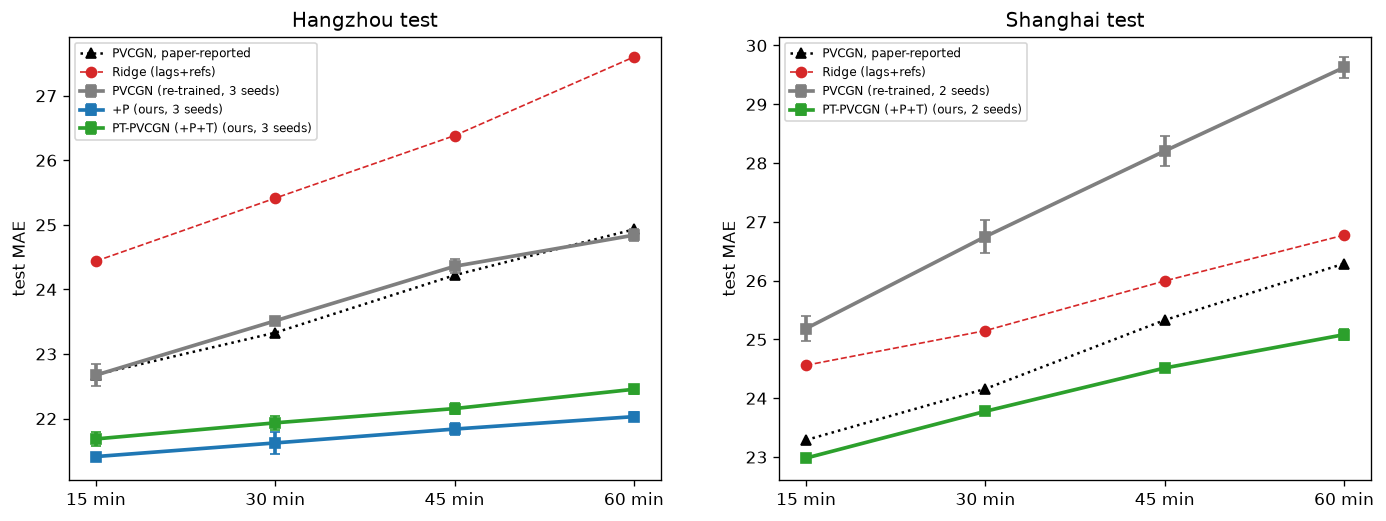
\includegraphics[width=\textwidth]{14_test_by_horizon.png}
\caption{Test MAE by horizon. Error bars: standard deviation over seeds.}
\label{fig:test}
\end{figure*}

\subsection{Ablation}
Table~\ref{tab:ablation} isolates the two components on HZMetro. The periodic inputs (P) account for the entire improvement: under the 200-epoch schedule +P obtains the lowest validation and test error (test MAE \hzP), and adding the calendar embeddings (T) does not help. The calendar embeddings were slightly helpful on validation with 100 epochs, which is why PT-PVCGN was designated the proposed model before the test; with the full schedule this benefit disappears. The table also shows a practical advantage of the periodic inputs: with only 100 epochs, +P and PT-PVCGN are within 0.33 MAE of (or better than) their 200-epoch validation error, whereas PVCGN is 1.87 MAE worse; under the 200-epoch schedule their best epochs (101--129) come shortly after the first learning-rate decay, PVCGN's (136--191) much later.

\begin{table}[t]
\centering
\caption{HZMetro ablation: MAE (mean $\pm$ std over 3 seeds) under the 200-epoch schedule used for all main results and under a shorter 100-epoch schedule. The final model was fixed on validation before the test evaluation.}
\label{tab:ablation}
\footnotesize
\begin{tabular}{lcccc}
\toprule
 & \multicolumn{2}{c}{200 epochs} & \multicolumn{2}{c}{100 epochs} \\
\cmidrule(lr){2-3}\cmidrule(lr){4-5}
Model & Val & Test & Val & Test \\
\midrule
PVCGN & 22.53\tiny{$\pm$0.15} & 23.85\tiny{$\pm$0.10} & 24.40\tiny{$\pm$0.36} & 25.84\tiny{$\pm$0.48} \\
+P & 20.93\tiny{$\pm$0.04} & 21.72\tiny{$\pm$0.09} & 21.26\tiny{$\pm$0.05} & 21.69\tiny{$\pm$0.03} \\
PT-PVCGN (+P+T) & 21.20\tiny{$\pm$0.12} & 22.06\tiny{$\pm$0.09} & 21.03\tiny{$\pm$0.04} & 21.86\tiny{$\pm$0.01} \\
\bottomrule
\end{tabular}
\end{table}

\subsection{Error analysis}
Table~\ref{tab:slices} and Fig.~\ref{fig:slices} break the test error down. PT-PVCGN is better than PVCGN at rush hours and on the busiest stations in both cities, and on SHMetro working days the gap is largest (\shWorkPT{} vs.\ \shWorkPV). Two calendar slices go the other way. On the Mid-Autumn holiday PT-PVCGN is worse than PVCGN (\shHolPT{} vs.\ \shHolPV), and on the make-up working Sunday it is worse as well (\shMakePT{} vs.\ \shMakePV). On these days the reference days are ordinary days whose pattern does not hold, and the model, having learned to trust its references, is misled; PVCGN, which only extrapolates the last hour, is not. On SHMetro non-working days the two models are close.

\begin{table*}[t]
\centering
\caption{Test MAE (mean over 4 horizons and over seeds) on operational slices. Rush hours: 07:30--09:30 and 17:30--19:30. Top-1/4: busiest quarter of stations by training ridership. SH holiday: Mid-Autumn Festival (Sep 15--17, 2016); SH make-up: Sunday Sep 18, 2016, an official working day.}
\label{tab:slices}
\footnotesize
\begin{tabular}{lcccccccc}
\toprule
Model & HZ rush & HZ top-1/4 & SH rush & SH top-1/4 & SH work & SH non-work & SH holiday & SH make-up \\
\midrule
Ridge & 30.56 & 47.77 & 34.10 & 48.21 & 26.04 & 24.77 & 24.41 & \textbf{29.23} \\
PVCGN (re-trained) & 31.39 & 40.65 & 38.86 & 48.22 & 29.61 & \textbf{23.10} & \textbf{21.48} & 29.41 \\
PT-PVCGN & \textbf{28.93} & \textbf{37.59} & \textbf{33.90} & \textbf{44.31} & \textbf{24.48} & 23.32 & 24.49 & 33.69 \\
\bottomrule
\end{tabular}
\end{table*}

\begin{figure*}[t]
\centering
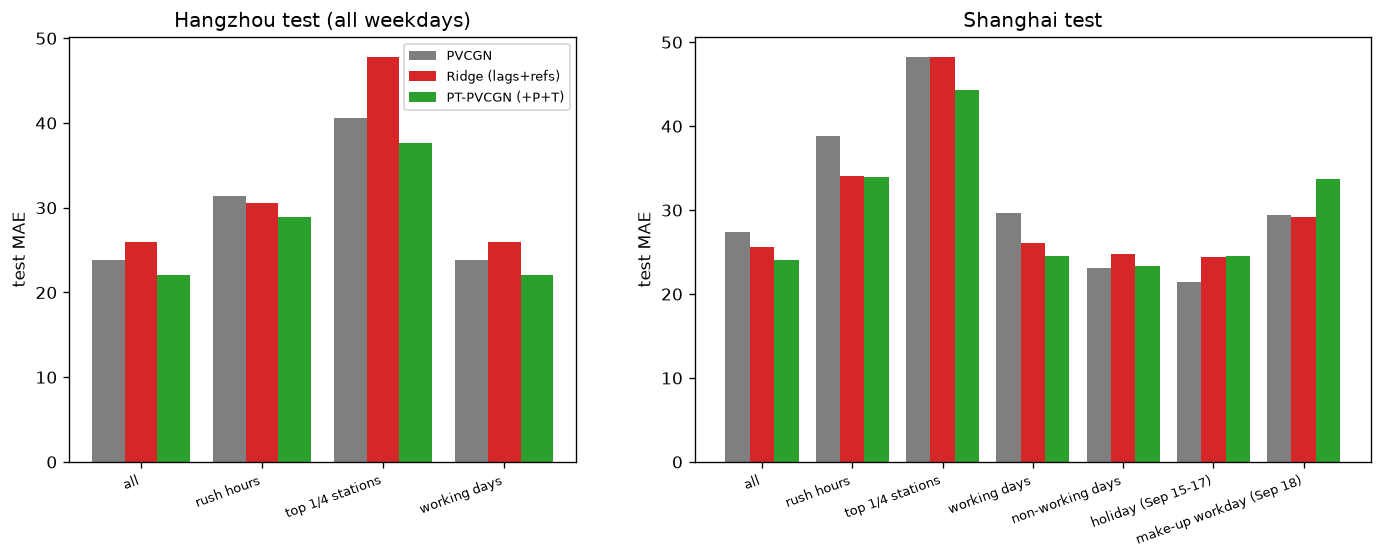
\includegraphics[width=\textwidth]{14_test_slices.png}
\caption{Test MAE by operational and calendar slice.}
\label{fig:slices}
\end{figure*}

\section{Discussion and Limitations}
The results support the research gap identified in PVCGN: a short look-back without periodic context leaves accuracy on the table, and the loss is largest exactly where operators need foresight---at longer horizons and in peaks. Several limitations qualify these findings. (i) SHMetro models were trained for 30 epochs only, against 200 in the original work. (ii) HZMetro covers a single month and its validation split contains only a weekend, so model selection rests on weekend behaviour while the test is on weekdays. (iii) The calendar embeddings brought no benefit with sufficient training; a simpler model with periodic inputs only is preferable in practice. (iv) The periodic references assume ordinary days; holidays and make-up working days degrade the forecasts, which suggests holiday-aware reference selection (e.g., the same holiday in a previous year) or falling back to recent-only models on irregular days. (v) We do not address OD-level prediction. Further natural extensions are time-varying virtual graphs---station similarity changes markedly between periods of the day (Fig.~\ref{fig:dyn})---and probabilistic forecasts.

\section{Conclusion}
We showed that PVCGN, a strong metro ridership forecaster, ignores the periodic structure that dominates metro demand, and that supplying it with the same time slots on comparable earlier days improves accuracy under a controlled, equal-budget comparison: \hzGain\% lower test MAE on HZMetro, rising to \hzGainSixty\% at 60 minutes, and a lower SHMetro error than the published PVCGN result despite a far shorter training budget. Periodic reference inputs, not calendar embeddings, carry this gain, and irregular calendar days remain the main failure mode.

\section*{Data and Code Availability}
The benchmarks are those released by~\cite{liu2022pvcgn}. Code, configurations, run logs and the scripts that generate every table: TODO(repository URL).

\section*{Acknowledgment}
TODO: acknowledge supervisor and institution. TODO: disclose the use of AI assistance as required by the target venue's policy.

\begin{figure}[t]
\centering
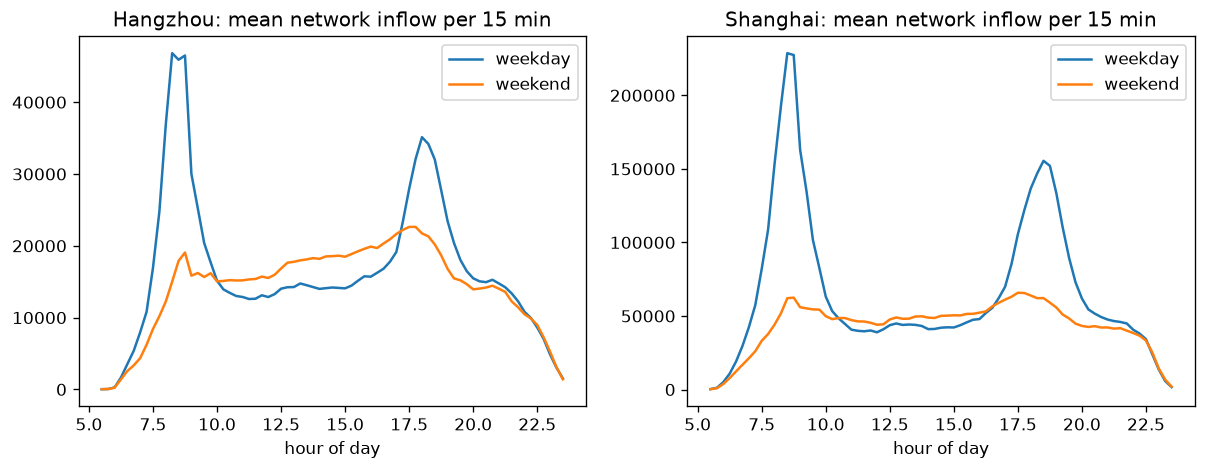
\includegraphics[width=\columnwidth]{02_daily_profile.png}
\caption{Mean network inflow per 15 minutes on weekdays and weekends.}
\label{fig:profile}
\end{figure}

\begin{figure}[t]
\centering
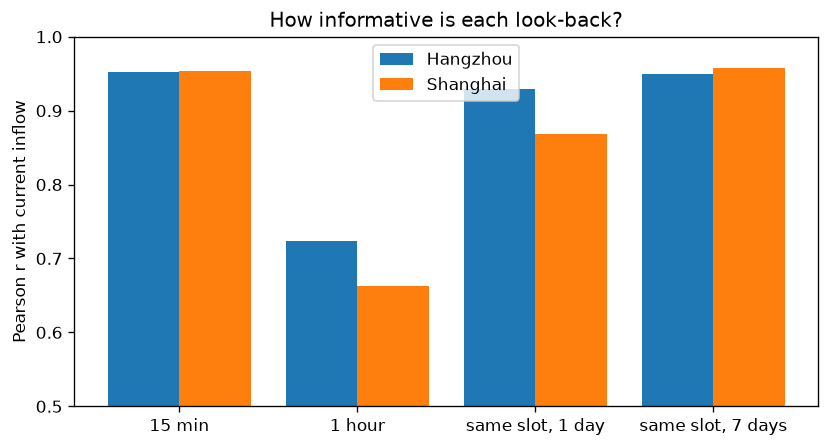
\includegraphics[width=\columnwidth]{02_periodicity_lags.png}
\caption{Correlation between current station inflow and each look-back.}
\label{fig:lags}
\end{figure}

\begin{figure}[t]
\centering
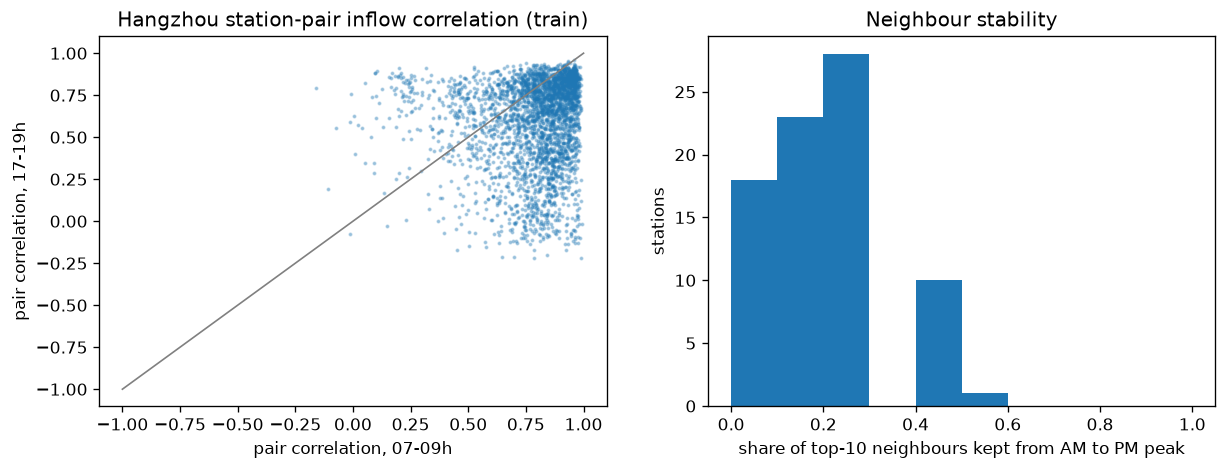
\includegraphics[width=\columnwidth]{02_dynamic_similarity.png}
\caption{HZMetro: station-pair inflow correlation in the morning vs.\ evening peak, and the share of each station's top-10 neighbours that persists.}
\label{fig:dyn}
\end{figure}

\bibliographystyle{IEEEtran}
\bibliography{refs}

\end{document}
